\section{Approach}
\subsection{Our Framework}
\begin{figure*}[h]
	\centering
	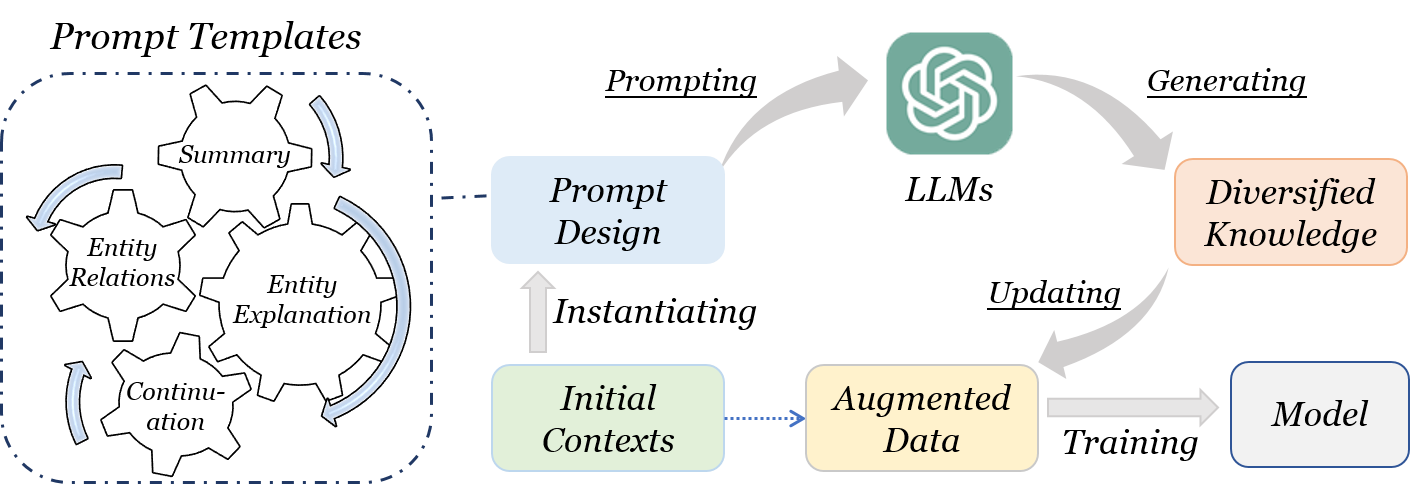
\includegraphics[width=18cm]{overview_v2.png}
	\caption{An overview of our automatic information augmentation framework. \textbf{(a) Step 1}: Interact with ChatGPT to Get Auxiliary Information. \textbf{(b) Step 2}: Distilling the Information and Injecting Them into Context \textbf{(c) Step 3}: Input the Augmented Context into Tagging Model}
	\label{fig:overview}
\end{figure*}   

 Given a question $Q_i \in Q = \{Q_1,...,Q_n\}$ and a context $C_i \in C = \{C_0,...,C_n\}$, where $C_i$ contains m tokens $c_0,..,c_m$, the objective of multi-span question answering is to identify a set of answer spans $A_i = \{a_0,...,a_s\}$ within the context. Here, each answer span $a_j \in A_i$ is represented as $a_j = c_{s_l},...,c_{e_l}$, where $s_l$ and $e_l$ denote the start and end positions of the l-th answer span, respectively.
 Following the observation of~\cite{li2022multispanqa}, We adopt the BIO tagging scheme to mark answer spans in the context where words are tagged as either part of the answer(\textbf{B}egin, \textbf{I}nside) or not (\textbf{O}ther). Formally, BIO tagging scheme is represented by a tag set $\tau = \{B, I, O\}$.

 Intuitively, large language models (LLMs) can serve as supplementary sources of external knowledge, compensating for the restricted semantic comprehension and limited information perception inherent in pre-trained language models). 
 We then propose a novel \textbf{G}enerative \textbf{I}nformation \textbf{A}ugme\textbf{NT}ation framework (GIANT) for multi-span question answering.
 GIANT employs a plug-and-play strategy to integrate the knowledge from large language models into the input layer of tagging models, built upon pre-trained language models.
 
 
 The overview of GIANT is depicted as \figref{fig:overview}.
 This process comprises the following steps:
 \textbf{1)Prompting}: constructing instruction templates to leverage language models for generating diversified data, involving entity elucidation, entity relationships, content continuation, and summarization.
 \textbf{2)Generating}: the large language model generating new knowledge based on the designed prompts.
 \textbf{3)Updating}: filtering the generated data, and combine it with metadata in different forms.
 \textbf{4)Training}: employing the knowledge-enhanced data to train a tagging model.

 In the following section, we will explore how GIANT utilizes a large language model to generate knowledge. Subsequently, we will delve into the methods employed by GIANT to filter these knowledge, amalgamate them into meta-context, and orchestrate ensemble strategies to leverage these knowledge effectively.

\textcolor{red}{提示的模板放在哪里描述比较好?}
\label{sec:prompt_construction}
\begin{figure*}[h]
	\centering
	\includegraphics[width=14.5cm]{Prompts_construction.png}
	\caption{Prompt Templates and it's Construction}
	\label{fig:prompt_template}
\end{figure*}   

\subsection{LLMs as Knowledge Source}
\label{sec:llm_as_knowledge_source}
 GIANT leverages a large language model as an external knowledge source, utilizing it to generate augmented data $K_i = \{E_i, S_i, R_i, F_i\}$ from multiple perspectives. Here, $E_i$ represents named entity elucidation, $R_i$ denotes entity relations, $S_i$ pertains to content summarization, and $F_i$ encompasses content continuation.

 Within these knowledge perspectives, named entity elucidation and entity relations provide factual knowledge, with GIANT synthesizing knowledge cues for the model by jointly injecting them into metadata.
 Summarization acts as a mechanism for information filtering, sieving and retaining entity interpretations and analyses of entity relationship, thereby ensuring augmentation efficiency. 
 Content continuation introduces relevant external knowledge by extending contextual content.
 
\subsubsection{LLMs as Content Summerizer}
 One of the pivotal factors in entity knowledge selection lies in ensuring that these entities exhibit semantic relevance within the specified context. The incorporation of disparate entity explanations and relationship analyses at the model's input layer may lead to the valueless augmentation of contexts, consequently impeding the model's learning.
 
 Utilizing the potent capabilities of large language models, we employ them to succinctly summarize the context $C_i$ into $S_i$, followed by extracting entities-based factual knowledge from $S_i$.
 By considering summarization as a knowledge filter, we can achieve information augmentation with greater efficiency.
 
\subsubsection{LLMs as Named Entity Elucidator}
\label{sec:LLMs as Named Entity Elucidator}
 The resolution of multi-span questions usually entails identifying named entities. This intricate task can be greatly improved by tapping into the specialized knowledge of named entities. This expertise directly aids the model in comprehending rare lexical items within its pre-training corpus and adapting to context-specific terminologies during fine-tuning. 
  
 While previous research has delved into entity knowledge either through training or direct application of fine-tuned NER models like spaCy and BERN2, these models have limitations stemming from their narrow training datasets and their tendency to solely provide extracted entities without contextualized meanings due to their inflexible design.  
 In comparison, generative large language models, endowed with advanced representation capabilities and abundant training data, present a promising avenue for achieving more precise and comprehensive entity delineations.
  
 GIANT utilizes a large language model to generate entity elucidation $E_i$ represented as $\{e_0,...,e_h\}$, from summary $S_i$ ,from summaries $S_i$ within each context $C_i$, where $i$ ranges from 1 to $n$. 
 Following this, it adopts a hybrid methodology integrating both regular expressions and semantic dependency analysis models, exemplified by spaCy, to parse the produced text.
 This systematic procedure culminates in the establishment of a ``Entity-Elucidation'' knowledge base oriented towards the elucidation of entities. 
 Furthermore, as \figref{fig:entity_insertion} presented, we seamlessly integrates the retrieved entity $e_t \in E_i$ mentioned within context $C_i$ by inserting its corresponding explanation immediately after the entity mention, significantly enriching the original text content while ensuring coherence and clarity are upheld.
 
\begin{figure*}[h]
	\centering
	\includegraphics[width=10cm]{EntityInsert.png}
	\caption{The Process of Inserting Entity Explanation into Context}
	\label{fig:entity_insertion}
\end{figure*}

\begin{figure*}[h]
	\centering
	\includegraphics[width=10cm]{RandomConcat.png}
	\caption{The Process of Concatenation of Original Context and Auxiliary Information}
	\label{fig:random_concatenate}
\end{figure*}  

\subsubsection{LLMs as Entity Relationship Extractor}
\label{sec:llm_as_relationship_extrator}
 Besides, understanding entity relations can also assist the model in untangling intricate logical relationships within complex context, thereby facilitating the clarification of interconnected concepts focused on the question-and-answering process.
 With the robust language comprehension capabilities, contextual sensitivity, and extensive external knowledge, large language models can adeptly capture entity associations within extensive contents and transform this structured knowledge into natural language expressions, thus integrating factual knowledge into the model in textual form. 
 Moreover, since entity interpretation and entity relationships are both factual knowledge, they naturally exhibit consistency, thus leading to their integration while GIANT injecting multiple knowledge into original context.
 
 After extracting the textual entity relationships $R_i$ from the summary $S_i$ of each context $C_i$, to maximize the interaction between context $C_i$ and relational knowledge $R_i$, we first calculate the ratio $r_l$, which is defined as the quotient of the cumulative length of the generated text $R_i$ and the total length of the original context $C_i$. 
 As depicted in \figref{fig:random_concatenate}, we subsequently partition the enhanced text $R_i$ and the original context $C_i$ into several segments, denoted as $\tilde{R_i} = \{\hat{r_1}, \hat{r_2}, ..., \hat{r_w}\}$ and $\tilde{C_i} = \{\hat{t_1}, \hat{t_2}, ..., \hat{t_w}\}$, respectively.
 After partitioning, the number of enhanced text segments $|\tilde{R_i}|$ equals the number of original context segments $|\tilde{C_i}|$, and the ratio of the length of each enhanced text segment $|t_i|$ to each original context segment $|c_i|$ is consistent with $r_l$. 
 Next, we maintain the order of the original context segments while shuffling the order of the enhanced text segments, represented as $R_i' = \{r_{\sigma(1)}, r_{\sigma(2)}, ..., r_{\sigma(m)}\}$, where $\sigma$ is a random permutation of the indices of the enhanced text segments. Then, we sequentially insert the shuffled enhanced text segments into the original text segments. This concatenation results in a new context $C' = \{c_1, r_{\sigma(1)}, c_2, r_{\sigma(2)}, ..., c_n, r_{\sigma(n)}\}$ enriched with relational knowledge.
 
	
\subsubsection{LLMs as Content Continuator}
\label{sec:llm_as_continuator}

 In addition to extracting and organizing knowledge from given contexts, we can enhance contexts by introducing external knowledge through the expansion of textual content. By continuing to write the original context, we enrich its content and themes, indirectly providing knowledge cues to models, thereby enabling model to learn more task-relevant information during fine-tuning.
 
 With extensive training data and parameters, large language models possess vast knowledge and domain backgrounds, exhibiting strong language expression capabilities and a deep understanding of context. Consequently, they can generate coherent and informative text extensions based on contexts. Such continuations not only improve text coherence but also enhance information content.
 
 The method of injecting extension knowledge is similar to injecting entity relationships into the original context. It involves randomly slicing the content continuation and inserting segmented text pieces into the original text, facilitating full interaction between the original and enhanced texts, which results in further enriching the semantics and content of the text.


\subsection{Knowledge Ensemble}
\label{sec:knowledge_ensemble}
 Various types of knowledge are closely interconnected. A deep understanding of one type of knowledge can facilitate comprehension across different types. For instance, grasping entity relationship analysis can significantly enhance entity interpretation. We have developed multiple strategies for combining knowledge, focusing on data ensemble and model ensemble. Our aim is to determine which combinations of knowledge yield better results and to improve overall effectiveness by optimizing knowledge organization methods.
\subsubsection{Data Ensemble}
\label{sec:data_ensemble}
 From the data ensemble perspective, we concurrently integrate various forms of knowledge into the metadata at the input layer of the model, thus learning a comprehensive knowledge enhancement model. The methodology for integrating each type of knowledge into the metadata during knowledge fusion aligns with the approach detailed in \secref{sec:llm_as_knowledge_source} specific to that type of knowledge. Given that entity interpretation and entity relationship analysis data stem from content summaries, a logical amalgamation emerges between summaries and the knowledge derived from entity interpretation and entity relationship analysis. Furthermore, considering that entity relationships and entity interpretation inherently embody factual knowledge centered on entities, we amalgamate them directly, conceptualizing it as a synthesis of summaries, entity interpretation, and entity relationship analysis. Ultimately, we can integrate content continuation knowledge into this tripartite fusion.
 Totally, we present two combinations of knowledge:
 $(a)$ integrating entity interpretation and entity relationship analysis, both derived from summaries, to mutually supplement factual knowledge;
 $(b)$ building upon $(a)$, incorporating content continuation knowledge.
 
 Illustrating through the exemplar combination $(a)$, we elucidate our methodology for knowledge amalgamation:
 \begin{enumerate}
 	\item \textbf{Integration of Entity Interpretation:} We first incorporate entity interpretation ($E_i$) immediately after the the entity mention within the original context $C_i$,with the result designated as $C_i'$.
 	\item \textbf{Refinement of Enhanced Text:} Employing a methodological approach encompassing slicing, shuffling, and strategic insertion, we imbue the enhanced text ($C_i'$), with  entity relationship analysis, thereby engendering an evolved iteration ($C_i''$).
 	\item \textbf{Model Augmentation:} Finally, the refined $C_i''$ is channeled into the model's input layer to learn a fusion model incorporating multiple forms of knowledge, which is utilized for both training and inference.
 \end{enumerate}
 Furthermore, for combination $(b)$, the process merely requires an additional step of inserting content continuation knowledge after step 2. All other procedures remain consistent with the exemplified approach, employing a injection method identical to that used for integrating entity relationship analysis $R_i$ data into entity-interpretation-enhanced context $C_i'$.
 

\subsubsection{Model Ensemble}
\label{sec:model_ensemble}
 From the model ensemble perspective, we first fine-tune multiple single-knowledge-enhanced question-answering models. During the prediction phase, each model performs token-based B/I/O classification on the context. Subsequently, for each token, we conduct a voting process on the prediction results from each model, selecting the category with the highest number of votes as the final classification result. In case of a tie, we compare the average probabilities of all categories provided by the models, and select the category with the higher average probability as the classification for the given token.
 
 Overall, we applied the aforementioned integration methods to two combinations for research purposes:$(a)$ combining factual knowledge (entity interpretation, entity relationships) with content continuation to compare the effectiveness of model ensemble methods versus data ensembles methods in knowledge fusion; and $(b)$ combining factual knowledge, content continuation, and other data augmentation methods (such as LIQUID) to investigate the compatibility between the model and other data augmentation methods.
 



